\chapter*{Introduction}
\label{chap:intro}
\addcontentsline{toc}{chapter}{\nameref{chap:intro}} %manually adding the unnumbered chapter to toc
In the last decades, the development of Machine Learning (ML) and Deep Learning (DL) techniques has contaminated every aspect of the scientific world, with interesting results in many different research fields. The biomedical field is no exception to this and a lot of promising applications are taking form, especially as Computer-Aided Detection (CAD) systems which are tools for the support for physicians during the diagnostic process. Medical doctors and the healthcare system in general collect a huge amount of data from patients during all the treatment, screening, and analysis activities in many different shapes, from anagraphical data to blood analysis to clinical images.

In fact in medicine, the study of images is ubiquitous and countless diagnostic procedures rely on it, such as X-ray imaging (CAT), nuclear imaging (SPECT, PET), Magnetic resonance, and visual inspection of histological specimens after biopsies. The branch of artificial intelligence in the biomedical field that handles image analysis to assist physicians in their clinical decisions goes under the name of Digital Pathology Image Analysis (DPIA).
In this thesis work, I want to focus on some of the beneficial aspects introduced by DPIA in the histological images analysis and some particular issues in the development of DL models able to handle this kind of procedure.

Nowadays the great majority of analysis of histological specimens occurs through visual inspection, carried out by highly qualified experts. Some analysis, as cancer detection, requires the ability to distinguish if a region of tissue is healthy or not with high precision in very wide specimens. This kind of procedure is typically very complex and requires prolonged times of analysis besides substantial economic efforts. Furthermore, the designated personnel for this type of analysis is often limited, leading to delicate issues of priority assignment while scheduling analysis, based on the estimated patient's clinical development. Some sort of support to this analysis procedure is therefore necessary.

The problem of recognizing regions with different features within an image and detect their borders is known in computer vision as the segmentation task, and it's quite widespread with countless different applications, allowing a sort of automatic image interpretation. In ML the segmentation problem is usually faced as a supervised task, hence the algorithm in order to be trained properly requires an appropriate quantity of pre-labeled images, from which learn the rules through which distinguish different regions. This means that the development of segmentation algorithms for a specific application, as would be the one on histological images, would require a lot of starting material, previously analyzed from the same qualified expert encharged of the visual inspection mentioned before. A human operator thus is required to manually track the boundaries, for example, between healthy and tumoral regions within a sample of tissue and to label them with their identity, as in Figure \ref{fig:man_seg}. The more the algorithm to train is complex the more starting material is required to adjust the model's parameters and reach the desired efficacy.

\begin{figure}
    \centering
    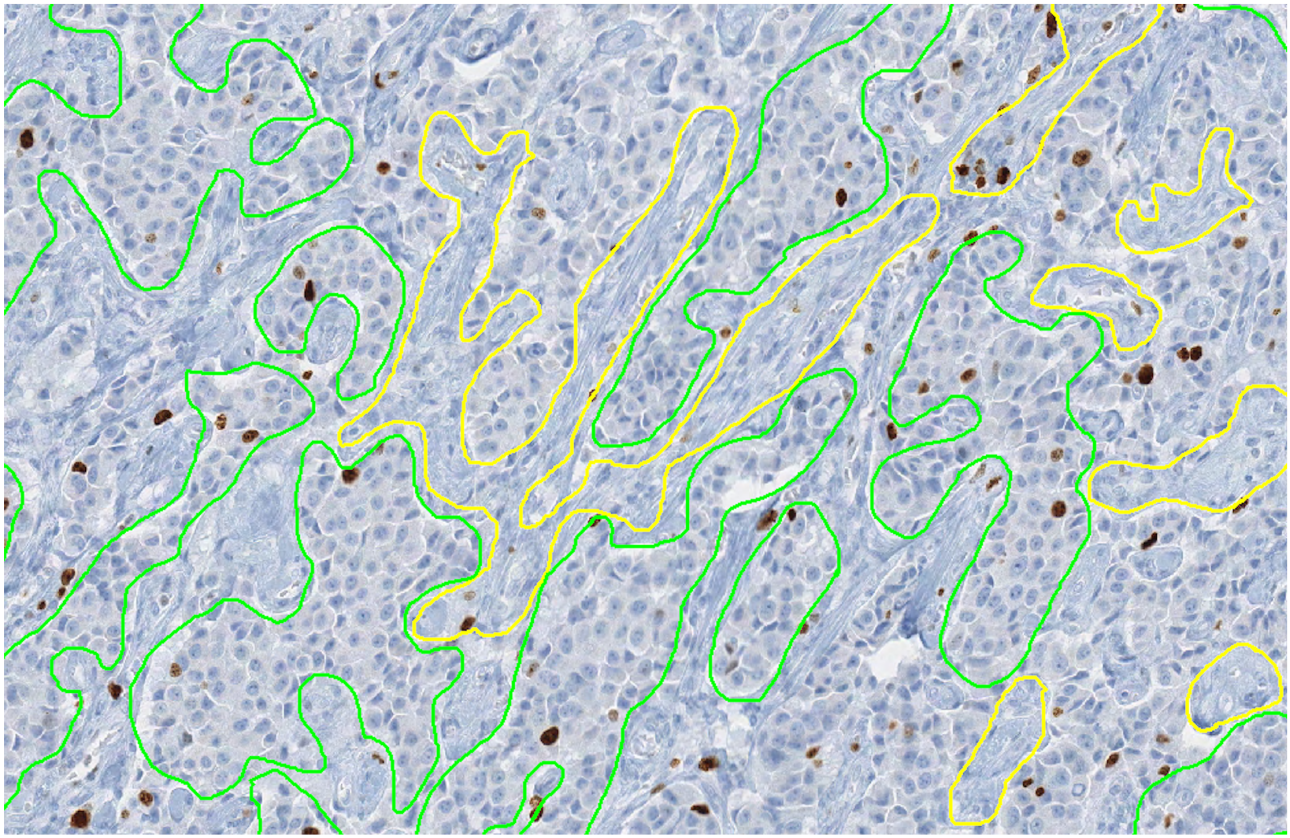
\includegraphics[width = 0.7\textwidth]{images/manual_seg}
    \caption{Interleaving of tumor (green annotation) and non-tumor (yellow annotation) regions \cite{Ki67}.}
    \label{fig:man_seg}
\end{figure}

The latest developed segmentation algorithms are based on DL techniques, hence based on the implementation of intricated Neural Networks (NN) which process the input images and produce the corresponding segmentation. Those models are typically very complex, with millions of parameters to adjust and tune, therefore they need a huge amount of pre-labeled images to learn their segmentation rules. This need for data is exactly the main focus of my thesis work. The shortage of ground truth images is indeed one of the toughest hurdles to overcome during the development of DL-based algorithms. Another important aspect to bear in mind is the quality of the ground truth material. It's impossible for humans to label boundaries of different regions with pixel-perfect precision, while for machines the more precise is the input the more effective is the resulting algorithm.

Different approaches have already been explored to overcome this problem, and they are mainly based on the generation of synthetic labeled data to use during the training phase. Some techniques achieve data augmentation manipulating already available images and then generating \textit{new} images, but as we will see this approach suffers from different issues. Here, I want to make an overview of some other interesting works on the generation of synthetic histological images, which have followed completely different paths and strategies from mine.

The first work I want to cite is a work from Ben Cheikh \textit{et al.} from 2017 \cite{10.1117/12.2254452}. In this work, they present a methodology for the generation of synthetic images of different types of breast carcinomas. They propose a method completely based on two-dimensional morphology operation, as successive image dilations and erosions. With the modulation of a very restricted number of parameters, regulating the abundance of the objects, their distribution in the image, and their shapes they are able to reconstruct realistic images reflecting different histological situations. In Figure \ref{fig:morpho_tripl} is shown an example of generated material besides a real histological H\&E stained sample. Starting from a generated segmentation mask which defines the \textit{tumoral pattern} the production of the synthetic image passes through successive steps, as the generation of characteristic collagen fibers around the structure, the injection of all the immune system cells, and some general
final refinements.

    \begin{figure}[ht]
        \centering
        \begin{subfigure}[t]{0.3\textwidth}
             \centering
             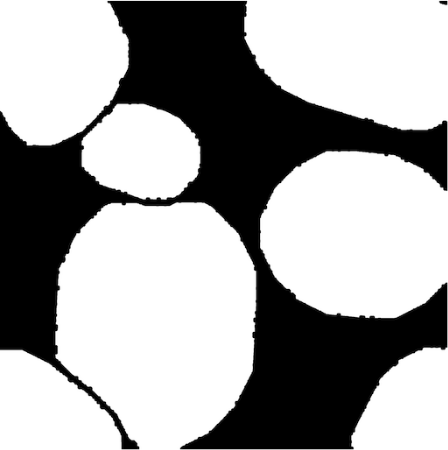
\includegraphics[width = \textwidth]{images/morpho_mask}
             \caption{}
             \label{fig:morpho_mask}
        \end{subfigure}
        \quad
        \begin{subfigure}[t]{0.3\textwidth}
             \centering
             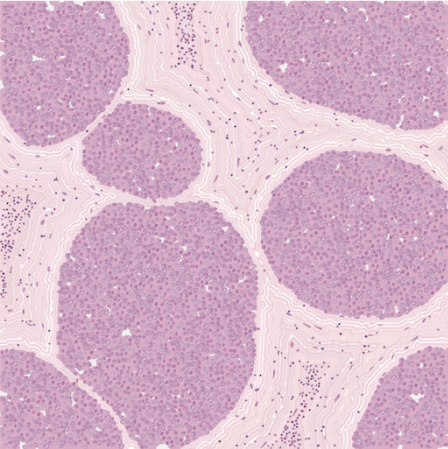
\includegraphics[width = \textwidth]{images/morpho_model}
             \caption{}
             \label{fig:morpho_model}
        \end{subfigure}
        \quad
        \begin{subfigure}[t]{0.3\textwidth}
             \centering
             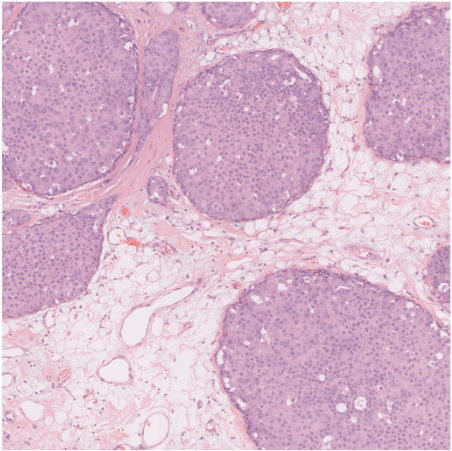
\includegraphics[width = \textwidth]{images/morpho_real}
             \caption{}
             \label{fig:morpho_real}
        \end{subfigure}
        \caption{Example of generated tumoral pattern (left), which acts as segmentation mask, of generated image (center) and a real example of the tissue to recreate, from \cite{10.1117/12.2254452}.}
        \label{fig:morpho_tripl}
    \end{figure}

The second work I want to mention is based on a DL-base technique, which approaches synthetic image generation using a specific cGAN architecture inspired to the ``U-net'' \cite{Senaras2018} model, as will be described in Figure \ref{fig:unet} in section \ref{ssec:soa_seg}. This model works with Ki67 stained samples of breast cancer tissue, and it is able to generate high-fidelity images starting from a given segmentation mask. Those starting segmentation masks tough are obtained through the processing of other real histological samples, via a nuclei-detection algorithm. The differences between real and synthetic samples are imperceptible, and the material generated in this work has effectively fooled experts, who qualified it has indistinguishable from the real one. In Figure \ref{fig:cgan_tripl} an example of a real image, a generated one, and their corresponding segmentation mask.

    \begin{figure}[t]
        \centering
        \begin{subfigure}[t]{0.3\textwidth}
             \centering
             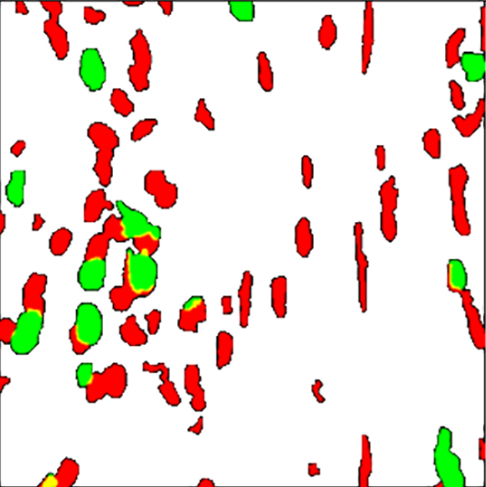
\includegraphics[width = \textwidth]{images/cgan_mask}
             \caption{}
             \label{fig:cgan_mask}
        \end{subfigure}
        \quad
        \begin{subfigure}[t]{0.3\textwidth}
             \centering
             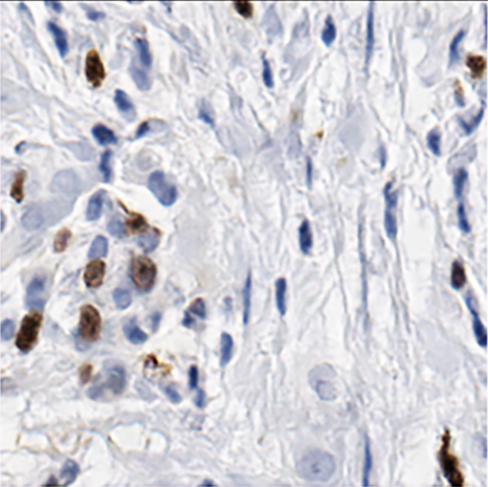
\includegraphics[width = \textwidth]{images/cgan_model}
             \caption{}
             \label{fig:cgan_model}
        \end{subfigure}
        \quad
        \begin{subfigure}[t]{0.3\textwidth}
             \centering
             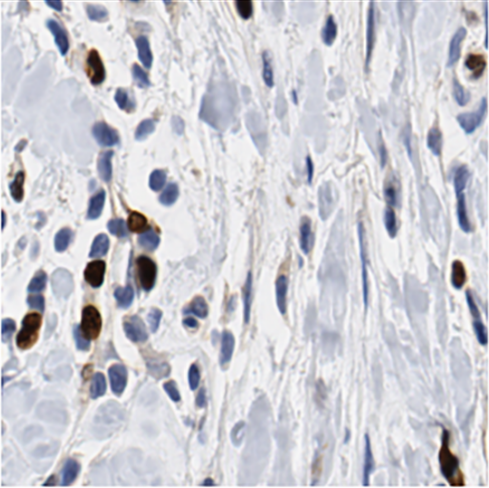
\includegraphics[width = \textwidth]{images/cgan_real}
             \caption{}
             \label{fig:cgan_real}
        \end{subfigure}
        \caption{Example of generated tumoral pattern (left), which acts as segmentation mask, of generated image (center) and a real example of the tissue to recreate, from \cite{Senaras2018}.}
        \label{fig:cgan_tripl}
    \end{figure}


Both of the two before-mentioned strategies produces realistic (or even perfect) results, but they are based onto considerations and analysis limited only to the aspect of the images. In the first work, the segmentation mask is produced in an almost full-random way, while in the second the segmentation mask is extracted starting from an actual real histological samples. The target of the present work instead lies in between those two approaches, and wants to produce randomized new images following a plausible modelization based on physical and histological considerations.

The technique I propose in this work follows a generation from scratch of entire datasets suitable for the training of new algorithms, based on the 3D modelization of a region of human tissue at the cellular level. The entire traditional sectioning process, which is made on real histological samples, is recreated virtually on this virtual model. This yields pairs of synthetic images with their corresponding ground-truth. Using this technique one would be able to collect sufficient material for the training (the entire phase or the preliminary part) of a model, overcoming the shortage of hand-labeled data. The 3D modeling of a region of particular human tissue is a very complex task, and it is almost impossible to capture all the physiological richness of a histological system. The models I implemented thus are inevitably less sophisticated respect the target biological structures. I'll show two models: one of pancreatic tissue and another of dermal tissue, besides all the tools I used and the choices I made during the designing phase.

Furthermore, since the image production passes through a wide and elaborated model, the resulting images contains a new level of semantic information that would not be encapturable otherwise. From the modelization is possible to reflect on the segmentation mask image the relationship information between nuclei and their belonging cells, or the basins of blood irrigation corresponding to every blood vessels and many other informations about the interrelationship of depicted elements. Moreover, achieving the right mastery of the modelization it is possible to reproduce different physiological states of the tissue like the healthy \textit{standard} configuration or different pathological situations, which reflect themselves as particular arrangments at cellular level. This aspect is of great interest, in fact there is a strong lack of real histological samples of healthy tissues samples, given the intrinsic nature of medical analysis. Biopsies are in general invasive procedure, and are tipically performed only when there is a concern for a pathological situation. Unless an erroneous evaluation, they typically collect a sample of non-healthy tissue. This method thus allow to collect an arbitrary number of samples in every interesting modelized condition, overcoming the problem of under-represented conditions.

In order to present organically all the steps of my work the thesis is organized in chapters as follows:

\begin{description}
    \item [1. Theoretical Background]. \hfill \\
    In this chapter, I will describe how real histological images are obtained and their digitalization process works. Afterward, I will introduce the reader to the Deep Learning framework, explaining the key elements of this discipline and how they work. Finally, I will dedicate a section to the image segmentation problem, and the state of the art of segmentation DL-based algorithms, with particular attention to the applications in the bio-medical field.

    \item [2. Technical Tools for Model Development]. \hfill \\
    I will dedicate this chapter to the thorough description of every technical tool I needed during the designing phase of this project. The development has required the harmonization of many different technologies and mathematical tools, some of which not so popular like quaternions, quasi-random number generation, Voronoi decomposition, and style transfer neural networks. In this chapter I will describe also the specialized algorithm I devised and implemented for the sectioning of an arbitrary polyhedron, which is the key element for the correct working of the virtual tomography technique described by this thesis work. As a conclusion for this chapter, I will describe the working environment I built for developing this project and I will mention all the code libraries I employed in my work.

    \item [3. Tissue Models Development]. \hfill \\
    This third chapter is the heart of the project. I will describe in detail all the steps necessary to create the two models, one of pancreatic tissue and the other of dermal tissue, and how I am able to produce the synthetic images. The first section is devoted to the modeling of the histological structures, while the second in entirely dedicated to the sectioning process and the subsequent refinements to the images.
\end{description}
